% =====================================================================
%  韓欣澄 — 推甄備審：簡歷（單頁）
%  編譯：xelatex resume.tex（需 xeCJK）
%  字型：中文 標楷體、英文 Times New Roman
%    - Windows 會用 DFKai-SB，Mac 會用 BiauKai；
%    - 都找不到時自動退回其他楷體／Times 相容字型，不會編譯失敗。
%    - 在 Overleaf 上使用：把標楷體字型檔（kaiu.ttf）上傳到專案，
%      並把下方 \setCJKmainfont 改成 [Path=./]{kaiu.ttf}。
% =====================================================================
\documentclass[10pt,a4paper]{article}
\usepackage[a4paper,top=1.2cm,bottom=1.1cm,left=1.5cm,right=1.5cm]{geometry}
\usepackage{fontspec}
\usepackage{xeCJK}
\usepackage{xcolor}
\usepackage{enumitem}
\usepackage{graphicx}
\usepackage{tikz}
\usepackage{pgfplots}
\usepackage{array}
\usepackage{colortbl}
\usepackage{tabularx}
\usepackage{hyperref}
\pgfplotsset{compat=1.17}

% ---------- 字型（自動偵測，依序嘗試）----------
\IfFontExistsTF{Times New Roman}
  {\setmainfont{Times New Roman}}
  {\setmainfont{Liberation Serif}}
\IfFontExistsTF{DFKai-SB}
  {\setCJKmainfont[AutoFakeBold=2.5]{DFKai-SB}}
  {\IfFontExistsTF{BiauKai}
    {\setCJKmainfont[AutoFakeBold=2.5]{BiauKai}}
    {\IfFontExistsTF{TW-Kai}
      {\setCJKmainfont[AutoFakeBold=2.5]{TW-Kai}}
      {\setCJKmainfont[AutoFakeBold=2.5]{AR PL UKai TW}}}}
\xeCJKsetup{CJKecglue={\hskip 0.2em plus 0.1em}}

% ---------- 顏色 ----------
\definecolor{navy}{RGB}{31,73,125}
\definecolor{ink}{RGB}{25,25,25}
\definecolor{hdrfill}{RGB}{221,228,238}
\color{ink}
\hypersetup{colorlinks=true,urlcolor=ink,linkcolor=ink,pdfborder={0 0 0}}

\setlength{\parindent}{0pt}
\pagestyle{empty}
\setlist[itemize]{leftmargin=1.1em,topsep=1pt,itemsep=0.5pt,parsep=0pt,
                  label={\scriptsize$\bullet$},before=\raggedright}

% ---------- 第 1 頁用的小工具 ----------
% 藍色區塊標題（含藍色底線）
\newcommand{\bsec}[1]{%
  \par\vspace{7.6pt}{\bfseries\fontsize{12.5}{14.5}\selectfont\color{navy}#1\par}%
  \nointerlineskip\vspace{2pt}\noindent\textcolor{navy}{\rule{\linewidth}{0.6pt}}\par
  \nointerlineskip\vspace{4pt}}
% 黑色區塊標題（含灰色底線）
\newcommand{\ksec}[1]{%
  \par\vspace{7.6pt}{\bfseries\fontsize{12.5}{14.5}\selectfont\color{navy}#1\par}%
  \nointerlineskip\vspace{2pt}\noindent\textcolor{navy}{\rule{\linewidth}{0.5pt}}\par
  \nointerlineskip\vspace{4pt}}
% 經歷條目：藍色粗體標題、下方副標
\newcommand{\etitle}[1]{\vspace{6.2pt}{\bfseries\fontsize{11}{13.6}\selectfont#1}\par}
\newcommand{\esub}[1]{{\fontsize{9.50}{12.35}\selectfont\raggedright #1\par}}
% 獎項條目
\newcommand{\award}[2]{\vspace{4.5pt}{\bfseries\fontsize{10.6}{13}\selectfont #1}\par
  \ifx\relax#2\relax\else{\fontsize{9.2}{11.5}\selectfont\raggedright #2\par}\fi}
\newcommand{\hl}[1]{{\color{navy}#1}}
\newcommand{\gsub}[1]{\par\vspace{7pt}{\bfseries\fontsize{10.8}{13}\selectfont #1\par}\nointerlineskip\vspace{1pt}\noindent{\color{black!35}\rule{\linewidth}{0.45pt}}\par\nointerlineskip\vspace{2pt}}
\newcommand{\hlb}[1]{{\bfseries\color{navy}#1}}

% ---------- 第 2 頁用的小工具 ----------
\newcommand{\asec}[1]{%
  \par\vspace{7pt}{\bfseries\fontsize{15}{18}\selectfont\color{navy}#1\par}%
  \nointerlineskip\vspace{3pt}\noindent\textcolor{navy}{\rule{\linewidth}{0.7pt}}\par
  \nointerlineskip\vspace{7pt}}
\newcommand{\asub}[1]{{\bfseries\fontsize{12.5}{15}\selectfont\color{navy}#1}\par\vspace{4pt}}

\begin{document}

% =====================================================================
%  第 1 頁：簡歷
% =====================================================================
\fontsize{9.70}{13.19}\selectfont

\newlength{\photoshift}\setlength{\photoshift}{1.2cm}
\noindent\begin{minipage}[c]{\dimexpr\linewidth-2.6cm-\photoshift\relax}
{\bfseries\fontsize{17}{20}\selectfont\color{navy} 韓欣澄\quad Hsin-Cheng Han}\par
\vspace{6pt}
{\bfseries\fontsize{10}{12}\selectfont 國立中央大學 資訊工程學系 ｜ 2023 -- Present}\par
\vspace{3pt}
{\fontsize{8.5}{10.5}\selectfont 0720samson@gmail.com \quad·\quad +886 909-728-676 \quad·\quad github.com/samson0720}\par
\end{minipage}\hfill
\begin{minipage}[c]{2.4cm}\raggedleft{\fboxsep=0pt\fboxrule=0.5pt\fcolorbox{black!35}{white}{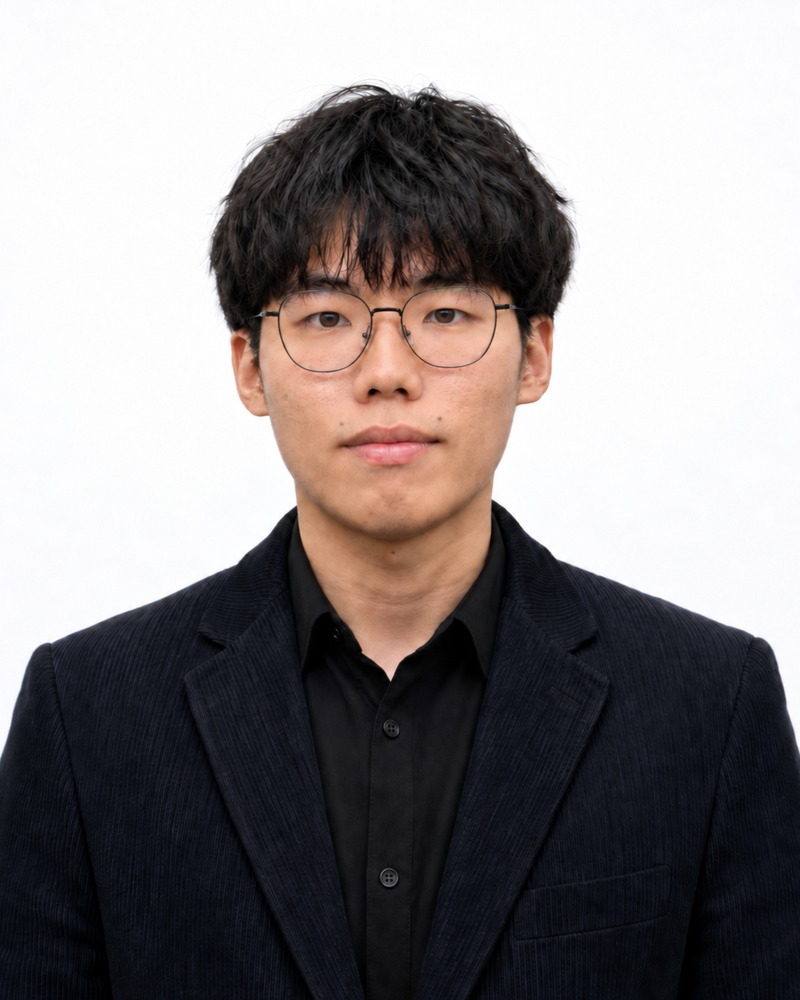
\includegraphics[height=2.9cm]{photos/photo.jpg}}}\end{minipage}\hspace*{\photoshift}\par
\nointerlineskip\vspace{5pt}\noindent\textcolor{black!45}{\rule{\linewidth}{0.5pt}}\par

\begin{minipage}[t]{0.595\linewidth}
\vspace{0pt}
\ksec{研究經歷}
\etitle{國科會大專生研究計畫｜Multimodal GraphRAG}
\esub{基於多模態圖譜推論的可溯源會議知識檢索系統\\ 中央資工大學部專題實驗競賽\ \hlb{佳作}}
\begin{itemize}
  \item 整合逐字稿、視覺資訊與投影片轉場，建構可溯源的多模態 GraphRAG 問答系統，使每則回覆能對應回原始素材。
\end{itemize}
\etitle{NTCIR-19 國際研討會論文（投稿中）}
\esub{Hierarchy-Constrained Decision Calibration and Decoding\quad 結果 10 月公布}
\begin{itemize}
  \item 固定 shared-encoder RoBERTa 之機率輸出，比較 calibration 與 17-state valid-state decoding；以 5-way rotating cross-fitting 及雙重資料切分檢驗跨文件泛化。
\end{itemize}

\ksec{競賽與專案}
\gsub{全國競賽}
\award{2025 客語 AI 應用黑客松｜\hl{冠軍}}{KaTCH 客語情境學習 App：以 Vision-Language Model 與生成式 AI，依情境即時生成學習內容}
\award{2025 土地銀行校園金融創意競賽｜\hl{全國冠軍}}{Green E Pass 綠易通：為土地銀行開發，輔助中小型企業 ESG 評估與轉型}
\award{AI CUP 2026｜ESG 承諾驗證\hl{前標}、桌球戰術預測\hl{佳作}}{教育部全國大專校院人工智慧競賽}
\gsub{國際競賽}
\award{生成式 AI 國際創新應用競賽｜\hl{佳作}}{2025\quad Format-Fluid：三階段 AI Chain，將複雜知識轉譯為 Podcast、漫畫與結構化摘要}
\gsub{校內競賽}
\award{校內網路應用創意競賽｜\hl{金牌獎}}{中央大學資訊工程學系}
\award{中央資工大學部專題實驗競賽｜\hl{佳作}}{Multimodal GraphRAG}
\gsub{成果展出}
\award{HLB 智慧驅鳥系統｜代表中央大學參展}{教育部新工程教育計畫成果交流活動；以物聯網與 AI 建構風力發電機的鳥類主動防護系統}

\ksec{領導與服務}
\etitle{教育部新工程教育計畫｜助教}
\esub{學院主題式課群建構計畫，參與 115 年期中海報審查暨成果交流活動}
\etitle{中央資工系學會｜學術部副部長}
\esub{共同創辦人，創立系學會學術部門}
\begin{itemize}
  \item 規劃 AWS Taipei、Trend Micro 企業參訪及升學／留學校友分享，累計逾 200 人次參與。
\end{itemize}
\etitle{資訊與社會服務 II｜組長}
\esub{帶隊拍攝資安相關影片，並上架於中央資工系官方頻道}
\end{minipage}%
\hfill
\begin{minipage}[t]{0.365\linewidth}
\vspace{0pt}
\bsec{學業表現}
{\fontsize{10}{13.4}\selectfont
\begin{tabular}{@{}p{0.5\linewidth}p{0.47\linewidth}@{}}
GPA & \textbf{4.19 / 4.30} \\
累計系排 & \textbf{13 / 117}\ {\fontsize{8.5}{10}\selectfont (11.1\%)} \\
近兩學期系排 & \textbf{2 / 108}\ {\fontsize{8.5}{10}\selectfont 班排 1} \\
書卷獎 & \textbf{2 次}\ {\fontsize{8.5}{10}\selectfont 114-1、114-2} \\
英文檢定 & \textbf{TOEIC 850} \\
\end{tabular}}\par
\gsub{資工核心科目}
{\fontsize{10}{13}\selectfont
\begin{tabular}{@{}p{0.29\linewidth}p{0.13\linewidth}p{0.29\linewidth}p{0.1\linewidth}@{}}
資料結構 & \textbf{A+} & 作業系統 & \textbf{A+} \\
演算法 & \textbf{A+} & 線性代數 & \textbf{A+} \\
計算機組織 & \textbf{A+} & 離散數學 & \textbf{A} \\
\end{tabular}}\par
\vspace{1pt}
{\fontsize{9}{11.5}\selectfont\raggedright 編譯器、軟體工程、軟體工程實務：滿分 100\\ 計算機結構：98\par}

\vspace{4pt}\bsec{實務經歷}
\etitle{Garmin｜Software Engineer Intern}
\begin{itemize}
  \item 參與 10+ APAC 對外與內部系統開發維護，涵蓋 Java、Spring Boot、legacy Grails、Vue.js 與資料處理流程。
  \item 以 Jenkins、Rancher / Kubernetes 執行 CI/CD 與 legacy system modernization，完整經歷 code review、測試驗證至正式環境部署之交付流程。
\end{itemize}
\etitle{AI CUP 全國競賽報名平台}
\esub{系統管理與網站開發}
\begin{itemize}
  \item 維運全國性報名平台（Django、Flask、PostgreSQL、MongoDB、Docker），負責上千名參賽者的報名資料，並支撐報名截止前的高併發流量。
  \item 與外部資安廠商協作系統更新與異常處理，異常率降低 50\% 以上。
\end{itemize}
\etitle{AWS Educate 雲端校園大使}
\esub{第九屆}
\etitle{帛瑀室內設計｜網站開發（接案）}
\esub{多頁式形象網站，從客戶需求訪談、設計、開發到上線獨立負責；HTML / CSS / JavaScript、EmailJS、Vercel。\\ silkyjade.com}
\etitle{中央大學環境工程研究所｜網管}
\esub{網路與系統管理：負責研究環境之伺服器與網路系統維運、帳號權限管理與異常排除。}

\vspace{4pt}\bsec{獎學金}
\award{中央大學優秀學生獎學金}{2026}
\award{一信文教基金會獎學金｜2 次}{2025、2026}


\end{minipage}

\end{document}
